
\documentclass[9pt]{report}
\usepackage[a4paper]{geometry}
\usepackage[myheadings]{fullpage}
\usepackage{fancyhdr}
\usepackage{lastpage}
\usepackage{graphicx, wrapfig, subcaption, setspace, booktabs}
\usepackage[T1]{fontenc}
\usepackage[font=small, labelfont=bf]{caption}
\usepackage{fourier}
\usepackage[protrusion=true, expansion=true]{microtype}
\usepackage[english]{babel}
\usepackage{sectsty}
\usepackage{url, lipsum}
\newcommand{\HRule}[1]{\rule{\linewidth}{#1}}
\doublespacing
\setcounter{tocdepth}{5}
\setcounter{secnumdepth}{5}
\usepackage{multirow}
\usepackage[table]{xcolor}
\usepackage{pdfpages}

%-------------------------------------------------------------------------------
% HEADER & FOOTER
%-------------------------------------------------------------------------------
\pagestyle{fancy}
\fancyhf{}
\setlength\headheight{15pt}
\fancyhead[R]{Assignment 1}
\fancyfoot[R]{Page \thepage\ of \pageref{LastPage}}
%-------------------------------------------------------------------------------
% TITLE PAGE
%-------------------------------------------------------------------------------

\begin{document}

\title{ \normalsize \textsc{Legacy System: Hailo Taxi Hailing App}
		\\ [2.0cm]
		\HRule{0.5pt} \\
		\LARGE \textbf{\uppercase{SOFTWARE ENGINEERING ASSIGNMENT 1}}
		\HRule{2pt} \\ [0.5cm]
		\normalsize \today \vspace*{5\baselineskip}}

\date{}

\author{
		Omphemetse Senna \\ 
		University of Pretoria \\ }

\maketitle
\newpage

%-------------------------------------------------------------------------------
% Section title formatting
\sectionfont{\scshape}
%-------------------------------------------------------------------------------

%-------------------------------------------------------------------------------
% BODY
%-------------------------------------------------------------------------------

\section*{1. Introduction}
%\subsection*{1. BACKGROUND INFORMATION}
\subsubsection*{1.1 BACKGROUND INFORMATION}
Hailo was a British tech-taxi hailing business\cite{intro}\cite{pessok} that connected taxi drivers and customers(passengers) through an Android and iOS mobile app\cite{mobile}, providing safe and convenient transportation\cite{app}. Founded in late 2010, it debuted in London in 2011 and then moved to North America\cite{citekey} by the end of 2012. The software enabled real-time tracking, secure payment processes, and wheelchair-accessible features.
\\\\
Hailo began as a taxi booking service that brought together customers with drivers in urban areas. However, by the end of 2014, it had ceased operations in North America due to heavy competition and a failure to create a strong relationship with New York taxi drivers. Other competitors, like Uber, dominated in more expensive cities and towns, while Hailo was unable to adjust to the market, eventually leading to its collapse. 
\\\\Hailo revolutionized\cite{riches} transportation by providing real-time tracking, safe payment methods, and wheelchair accessibility\cite{intro}. The Hailo mobile application was popular in the transportation industry, notably among taxi drivers who supplied transportation to consumers.

\subsection*{1.2 PROBLEM STATEMENT}
During its existence, the Hailo app encountered challenges including competition from other transportation companies, difficulty adapting to national market needs and regulations, and dealing with legal issues such as lawsuits. These difficulties restricted the mobile application's expansion and durability in the sector of transportation, emphasising the importance of innovation, careful planning, and adherence to legislation for market success.
\subsection*{1.3 DEFINITION OF SCOPE}
This project aims to improve the Hailo app by adding features such as a cloud database, machine learning, geolocation services, social media platforms, and in-app messaging. Cloud databases and machine learning will make it possible for continuous updates, data analysis for performance monitoring, and recommendations on where to focus and what to improve in order to advance further in the market. Social media will be used for marketing and advertising the application and the geolocation services that enable precise pick-up and drop-off locations, real-time traffic information for informed decision-making, and messaging within the app for customer-driver contact.
\section*{2. USER CHARACTERISTICS}
The intended users for the Hailo app are diversified, including customers, drivers, administrators, data scientists(analytics):
\begin{itemize}
\item \textbf{Customers:}
    \begin{itemize}
        \item \textbf{Education}: Customers are assumed to have smartphone expertise and technical skills because the mobile application is designed to be simple to use and accessible to a wide range of users. The customer would use the system to request services (rides), follow driver locations, and make payments.
        \item \textbf{Age}: Customers must be at least 12 years old, unless a parent requests services on their behalf. In such circumstances, the parent should show their registered ID to the driver.
        \item \textbf{Physicality}: The Hailo app should be designed to be accessible and user-friendly for all, including people with disabilities. This includes wheelchair options, audio descriptions, adaptable text sizes, and voice command capabilities, which ensure that every customer can travel simply, communicate with drivers, and navigate their journeys. Prioritising inclusion in app design can help build a more accessible transport service for individuals with disabilities.
        \item \textbf{Gender}: Any gender can request services.
    \end{itemize}

\item \textbf{Drivers:}
    \begin{itemize}
        \item \textbf{Education}: Drivers must have an educational foundation that includes knowledge of geography and basic finance, as well as a basic understanding of mobile devices and navigation systems.
        \item \textbf{Experience}: Drivers should have at least three years of driving experience, as they will be using the system to handle trip requests, find pick-up and drop-off locations, manage their schedules, and track payments, particularly cash.
        \item \textbf{Age}: expected should be above 18 and below 60. 
        \item \textbf{Physicality}: The Hailo app should provide accessibility features such as voice commands, larger text sizes, and colour contrast adjustments to ensure that all drivers, regardless of impairment, can efficiently use the platform for tasks such as service requests, navigation, and calendar management.
        \item \textbf{Gender}: Any gender can request services.
    \end{itemize}

\item \textbf{Admin:}
    \begin{itemize}
        \item \textbf{Education}: Administrators are expected to have higher technical expertise, as they would use technological tools to administer accounts for users and monitor system operations. To increase efficiency, monitor performance data and apply updates and enhancements.
        \item \textbf{Age}: should be below 65.
        \item \textbf{Physicality}: Admin with disability are allowed to apply.
        \item \textbf{Gender}: Both Male and Females are allowed.
    \end{itemize}

\item \textbf{Data Scientists/Analytics:}
    \begin{itemize}
        \item \textbf{Education}: Degrees in data science, analytics, or similar fields are among the educational prerequisites.
        \item \textbf{Experience or expertise:} Proficiency in data visualisation, machine learning, and database management are among the expertise sets required to analyse large amounts of data, identify trends, develop demand forecasting models, and increase productivity in the on-demand transportation industry, promoting innovation and business growth.
        \item \textbf{Age}: should be below 65 years.
        \item \textbf{Gender}: Any gender can request services.
    \end{itemize}
\end{itemize}

\section*{3. USER STORY AND FUNCTIONAL REQUIREMENTS:}
%----------------------------------------customer ---------------------------------------
\subsection*{U1 - Use Case Name: Sign up}
\textbf{Actor(s):} Customer (Primary) and Driver(Primary)
\textbf{\\User Story:} \\The on-boarding process allows the riders to be able to utilise the system's functionalities. During this initial phase, user identities are created and are unique for each new user, and security protocols are put in place to prioritise safety.\\In the system, there are two types of sign-ups: for customers (U1.1) and for drivers (U1.2).
\begin{itemize}
    \item \textbf{For U1.1}, customers have the option to set up an account by entering their personal information. This allows them to request services (ride) and ensures data accuracy.
    \item \textbf{For U1.2}, drivers have the option to register by submitting their personal information, vehicle details, and licence information. The details entered during registration will be stored in a cloud-based database.
\end{itemize}
\textbf{Input data:}
\begin{enumerate}
    \item Username.
    \item Surname.
    \item First name.
    \item Gender.
    \item Email Address.
    \item Cell Phone number.
    \item Password.
    \item Date of birth
\end{enumerate}
\textbf{Input data - Extension for Drivers:}
\begin{enumerate}
    \item Licence Information.
    \item Vehicle Information.
    \item Address.
    \item Documents(Licence documents, Proof of address).
\end{enumerate}
\textbf{Functional Requirements:}
\begin{itemize}
    \item \textbf{FR1.1:} If the username, email address, and phone number already exist in the database, the system should not register the new user account.
    \item \textbf{FR1.2:} The system should be able to create a new account for the user and validate the provided information.
    \item \textbf{FR1.3:} The system should allow the users to register an account on the system using their phone number, email address, or Google account.
    \item \textbf{FR1.4:} The system should be able to send an account confirmation link or code on the email or on text message.
    \item \textbf{FR1.5:} The system should be able to input user passwords and other personal information and be able to confirm the password entered.
    \item \textbf{FR1.6:} In order to guarantee account security and authenticate user credentials, the system must be able to incorporate a verification process.
    \item \textbf{FR1.7:} The system should have an option to enter payment details for easy client transactions.
    \item \textbf{FR1.8:} The system should be able to upload the documents from the user (Driver).
\end{itemize}
\textbf{Extensions:}
\begin{itemize}
    \item \textbf{FR1.9:} If the customer enters invalid information, the system should prompts for correction.
    \item \textbf{FR1.10:} If the verification code or link on the email or cell phone message is not sent, the user can resend to receive one.
\end{itemize}
\textbf{Pre-Condition:}
\begin{itemize}
    \item The user must have access to the internet before interacting with the system.
    \item The user must have or know their cellphone number, email, username to use, and date of birth to register an account.
\end{itemize}
\textbf{Post- Condition:} 
\begin{itemize}
    \item The user have successfully created the new account on the system up.
    \item The user received an email (or optionally text message) for confirmation of the email account.
    \item The user's account is verified, and they can start using the system.
    \item The user's(driver) account is verified and the background checks have been made.
\end{itemize}


%----------------------------------------Sign In customer---------------------------------------
\subsection*{U2 - Use Case Name: Sign in}
\textbf{Actor(s):} customer (Primary) and Driver (Primary)
\textbf{\\User Story:} 
There are two sign-ins in the system (U3 and U3):\\
Registered users (drivers and customers) can log in to their accounts using their credentials.
\begin{itemize}
    \item Allows the customer-user to access their account, which can be used by the customer to login to the app and request services such as booking a ride, viewing history, rating drivers, and making payments. 
    \item Allows the driver-user to access their account, which can be used by the driver to login to the app and provide service. Drivers can accept or reject ride requests from customers and can also view history, ratings, and update their availability.
\end{itemize}


\textbf{\\Input data:}
\begin{enumerate}
    \item Email Address/Username/cellphone number/Google account
    \item Password
\end{enumerate}
\textbf{Functional Requirements:}
\begin{itemize}
    \item \textbf{FR2.1:} The system must have "Remember Me" functionality to facilitate faster logins for returning and frequent users.
    \item \textbf{FR2.2:} An instant notification system for important updates on the system.
    \item \textbf{FR2.3:} In a situation where login credentials are forgotten, the system needs to include an link for redirecting the users to a page of recover passwords. 
    \item \textbf{FR2.4:} Secure authentication techniques, including two-factor authentication or password-based login, must be implemented in the system.
    \item \textbf{FR2.5:} Verification process to verify user credentials and ensure compliance with regulations. 
    \item \textbf{FR2.6:} The system must allow the user to have access to their service history upon successful login.
    \item \textbf{FR2.7:} The system must have the ability to set availability status (online or offline) for receiving ride requests from the user (driver).
    \item \textbf{FR2.8:} The system prompts the user to enter their email address, cellphone number or user name and passwords.
    \item \textbf{FR2.9:} Logging in date and time is recorded upon successful login.
\end{itemize}
\textbf{Extensions:}
\begin{itemize}
    \item \textbf{FR2.10:} If the user enters incorrect credentials, the system prompts for correction message to the user to re-enter details.
    \item \textbf{FR2.11:}  For faster access, a Google account login option must be included in the system.
    \item \textbf{FR2.12:}  reset password when the user forgot it.
\end{itemize}
\textbf{Pre-Condition:} 
\begin{itemize}
    \item The user must have access to the internet before interacting with the system.
\end{itemize}
\textbf{Post-Condition:}
\begin{itemize}
    \item The user have successfully logged in on the system.
    \item The security measures are in place to secure user's login information upon successful login.
    \item The user (driver) can access the driver’s portal for ride requests.
    \item The user (customer) can access the customer’s portal for service requests.
\end{itemize}

%----------------------------------------Request password---------------------------------------
\subsection*{U3 - Use Case Name: Request password}
\textbf{Actor(s):} Driver (Primary), customer (Primary)
\textbf{\\User Story:} \\ Registered users (customers and drivers) can reset and update their passwords if they forget them or want to secure their accounts. After resetting the password, the user can gain access to the system.
\textbf{\\Input data:}
\begin{enumerate}
    \item Email Address or cellphone number.
    \item Identity Number.
\end{enumerate}
\textbf{Functional Requirements:}
\\\textbf{FR3.1:} The user launches the system and chooses the Forgot Password option.
\\\textbf{F3.2:} Accepts email addresses, cell phone numbers, and the user's identification number as inputs.
\\\textbf{F3.3:} Authenticates the input credentials to verify if the account exists in the database and matches.
\\\textbf{F3.4:} The system has to forward a password reset link to the user's email address or phone number.
\\\textbf{F3.5:} Sends the link to the user, and when clicked, the system must route the user to the page where they can input their new password.
\\\textbf{F3.6:} Validate the new password and submit it.
\\\textbf{F3.7:} A successful password reset requires the system to change the password in the database and notify the user by email or cell phone message.\\\\
\textbf{Extensions:}
\\ \textbf{FR3.8:} If the user enters a password that does not meet the system's requirements, the system shows a correction message and asks the user to reenter the password.\\
\textbf{Pre-Condition:} 
\begin{itemize}
    \item The user must have downloaded and installed the system and additionally possess an active connection to the internet.
    \item The user forgot the system password.
\end{itemize}
\textbf{Post-Condition:} 
\begin{itemize}
    \item After successfully resetting their password, the user can log in to the system using their new credentials.
    \item Users can view the app's services and history.
    \item user can request rides through the driver site.
    \item User login information is secure.
\end{itemize}


%----------------------------------------Request Service (Ride)---------------------------------------
\subsection*{U4 - Use Case Name: Request Service (Ride)}
\textbf{Actor(s):} customer (Primary), Bank (secondary)
\textbf{\\User Story:}
\\User (customers) are given the opportunity to enter the system and request for services (rides). Once a user, which is the customer logs in they can request services, have various payment options available. They are able to see their pick up spot, on a map based on geo-location. After the service is completed users will receive a prompt to rate the driver. Will be sent a payment receipt after service. \\ The bank is a third-party that accepts payments made by the customer such as EFT, vouchers and using bank card.


\textbf{\\Input data:}
\begin{enumerate}
    \item Pick-up location.
    \item Drop-off location.
\end{enumerate}
\textbf{Functional Requirements:}
\begin{itemize}
    \item \textbf{F4.1:} The system must allow the user to specify the pick-up and drop-off locations.
    \item \textbf{F4.2:} The system estimates service rates based on location.
    \item \textbf{F4.3:} The system must be able to locate the precise locations specified by the user.
    \item \textbf{F4.4:} The system must indicate available nearby drivers, as well as the drivers' expected arrival times to the customer and the drop-off site.
    \item \textbf{F4.5:} The system must allow customers to select their preferred car and display the amount of service.
    \item \textbf{F4.6:} The system must allow the customer to select the mode of payment.
    \item \textbf{F4.7:} The system displays the details of the driver who accepted the customer's service request.
    \item \textbf{F4.8:} In-app messaging and calls allow customers and users to communicate directly.
    \item \textbf{F4.9:} In-app messaging and in-app call feature for communication between the customer and the user.
    \item \textbf{F4.10:} The system must alert the user (customer) when the driver arrives at the pickup and drop-off locations.
    \item \textbf{F4.11:} The system must allow users to rate the driver and provide tips.
\end{itemize}
\textbf{Extensions:}
\begin{itemize}
    \item \textbf{F4.12:} If the system cannot find the entered location, it should display a possible location and allow the consumer to enter the closest place to the drop-off location.
    \item \textbf{F4.13:} A success notification appears when the customer gets into the driver's car and is ready to depart the starting point, as well as after the ride is concluded once the drop-off location has been reached.
    \item \textbf{F4.14.} The system can display a notification for rating drivers.
    \item \textbf{F4.15.} The system allows user to change the driver drivers.
    \item \textbf{F4.15.} The system allows user to cancel service requested..
\end{itemize}
\textbf{Pre-Condition:} 
\begin{itemize}
    \item The user must have access to the internet before interacting with the system.
\end{itemize}
\textbf{Post-Condition:} 
\begin{itemize}
    \item The user successfully requests a ride through the system, and the driver accepts the request.
    \item The user can track the driver's location to the pick-up site, the ride's progress, and the drop-off location.
    \item The customer can rate the driver's service and leave a tip.
    \item The user made payments.
\end{itemize}

%----------------------------------------Provide Service (Ride)---------------------------------------
\subsection*{U5 - Use Case Name: Accept and Provide Service (Ride)}
\textbf{Actor(s):} Driver (Primary), Google(secondary)
\textbf{\\User Story:}
\\Permits the driver to access the system, accept customer requests, and deliver services (riding).
Geo-location can optimise routes by displaying traffic and construction, as well as providing quickest pathways to client destinations (pick-up and drop-off locations). \\Google will be used as one of the route optimization tool if there is no built in route-optimization.

\textbf{\\Functional Requirements:}
\begin{itemize}
    \item \textbf{FR5.1:} The user has successfully accessed the system, and the system permits the driver to navigate the service portal or page.
    \item \textbf{FR5.2:} The system allows the driver to identify and update their availability (whether online or offline).
    \item \textbf{FR5.3:} The system must allow the driver to get the customer's trip request notification and report, which includes the amount, pick-up location, projected arrival time to the customer and drop-off destination, and the method of payment.
    \item \textbf{FR5.4:} The system must allow the driver to accept or decline the customer's ride request.
    \item \textbf{FR5.5:} Allows the user to navigate to the pickup location of the customer's geo-location navigator.
    \item \textbf{FR5.6:} The system must allow the driver to alert the customer through the system when they arrive at the pickup location.
    \item \textbf{FR5.7:} When the user selects cash as a payment method, the system must finish the rides in the mobile app and prompt a message informing the driver if he or she took the payment.
\end{itemize}
\textbf{Extensions:}
\begin{itemize}
    \item \textbf{FR5.8:} When the driver arrives at the drop-off location and completes the transaction, a successful message appears.
    \item \textbf{FR5.9:} The system allows the user to cancel service.
\end{itemize}
\textbf{Pre-Condition:} 
\begin{itemize}
    \item The driver has logged into the system and is ready to give services to consumers.
    \item In order to use the system, the user must have a steady network connection.
\end{itemize}
\textbf{Post-Condition:} 
\begin{itemize}
    \item The driver effectively provides a ride to the consumer through the application.
    \item The driver refreshes their state so that the system can detect and assign customers.
    \item The driver either earned rates and tips for the service or did not.
\end{itemize}

%----------------------------------------Source data---------------------------------------
\subsection*{U6 - Use Case Name:  Source and Extract Data}
\textbf{Actor(s):} Data Scientist/Analyst (Primary)
\textbf{\\User Story:}\\enables the user to acquire raw data on customers and drivers, locations, politics, markets, and competitors from many sources and save it in a database for analysis to help enhance the business.
\textbf{\\Functional Requirements:}
\begin{itemize}
    \item \textbf{FR6.1:} The user integrates with a database to collect user information.
    \item \textbf{FR6.2:} The system enables data extraction by collecting structured and unstructured data from various data sources.
    \item \textbf{FR6.3} The system allows data to be categorised into categories and saved in a database.
    \item \textbf{FR6.4} The system supports many data pipelines for effective data collection.
    \item \textbf{FR6.5} Allows data encryption and secure storage processes.
\end{itemize}
\textbf{Extensions:}
\begin{itemize}
    \item \textbf{FR6.6.} Set pipelines or external data sources to enhance the analysis.
    \item \textbf{FR6.7.} Message of success or failure to store data.
\end{itemize}
\textbf{Pre-Condition:}
\begin{itemize}
    \item The user possess access and permission to relevant data sources.
    \item The user have access to appropriate data repositories for storing data.
\end{itemize}
\textbf{Post-Condition:} 
\begin{itemize}
    \item The user has successfully sourced the data.
    \item The user successfully stored data across many repositories.
\end{itemize}

%----------------------------------------Analyse data---------------------------------------
\subsection*{U7 - Use Case Name:  Analyse Data}
\textbf{Actor(s):} Data Scientist/Analyst (Primary), Stakeholder(secondary)
\textbf{\\User Story:} \\The user evaluates data from customers, drivers, and other sources to improve business operations. It also entails cleaning raw data, analysing customer behaviours, anticipating demand, optimising pricing, and implementing various machine learning models to improve operational efficiency and other aspects of the business that require improvement.
\textbf{\\Functional Requirements:}
\begin{itemize}
    \item \textbf{FR7.1:} The system provides access of raw data stored from the database.
    \item \textbf{FR7.2:} Clean data is stored in the database and ready for analysis.
    \item \textbf{FR7.3:} The system allows data visualisation and creates dashboards and reports.
    \item \textbf{FR7.4:} The system supports statistical analysis and machine learning methods for predictive modelling and data forecasting.
    \item \textbf{FR7.5:} Improve operational efficiency.
    \item \textbf{FR7.6:} The data scientist employs several models to forecast demand for services at various locations and periods.
    \item \textbf{FR7.7:} Optimise pricing techniques.
\end{itemize}
\textbf{Extensions:}
\begin{itemize}
    \item \textbf{FR7.8:} The user engage with external partners to provide data and insights.
\end{itemize}
\textbf{Pre-Condition:} 
\begin{itemize}
    \item The user has access to relevant data repositories, which hold data.
    \item The user has access to analytical tools.
\end{itemize}
\textbf{Post-Condition:} 
\begin{itemize}
    \item The results of the analysis are collected, and the user creates reports.
    \item Businesses can use insights to make better decisions.
    \item The user reported their findings to the stakeholders.
    \item The user enhanced the client experience while also advancing the business.
\end{itemize}


%----------------------------------------MANAGE USERS---------------------------------------
\subsection*{U8 - Use Case Name: MANAGE USERS}
\textbf{Actor(s):} Admin (Primary) and Stakeholder (Secondary)
\textbf{\\Summary Description:} \\ The user (admin) can manage active accounts, user profiles, and procedures on the system. It also allows the administrator to connect with drivers and customers who are experiencing system troubles. The user can update, add, and delete customer and driver profiles, as well as compile and deliver reports to stakeholders.\\
\textbf{Functional Requirements:}
\begin{itemize}
    \item \textbf{FR8.1:} permits the user to verify a driver's information and approve their application.
    \item \textbf{FR8.2:} The system enables the user to manage customer and driver complaints and feedback.
    \item \textbf{FR8.3} User account administration (activating and deactivating accounts).
    \item \textbf{FR8.4:} The system enables the user to communicate with clients and drivers as needed and provide support.
    \item \textbf{FR8.5:} Dashboards for transaction and account reporting.
    \item \textbf{FR8.6} Functionality for monitoring and analysing user actions.
    \item \textbf{FR8.7} Generate profile reports.
\end{itemize}
\textbf{Extensions:}
\begin{itemize}
    \item \textbf{FR8.8.} The system must allow the user to delete, add, and modify users' profiles.
    \item \textbf{FR8.9.} Resolve any issues that arise.
\end{itemize}
\textbf{Pre-Condition:} 
\begin{itemize}
    \item The user has the required access.
    \item The user maintains communication channels with both customers and drivers.
    \item The user understands the company's policies and processes.
\end{itemize}
\textbf{Post-Condition:} 
\begin{itemize}
    \item User (Customer and Driver) profiles are updated, added, or deleted, and any issues are addressed.
    \item Drivers have been verified and approved on the site.
    \item Reports are created or generated.
\end{itemize}

%----------------------------------------MAINTAIN APPLICATION---------------------------------------
\subsection*{U9 - Use Case Name: MAINTAIN APPLICATION}
\textbf{Actor(s):} Admin (Primary) and Stakeholder (Secondary)
\textbf{\\Summary Description:} \\Users can execute maintenance assignments to maintain optimal system performance. After making changes to the system, the user can update it, add new features, shut the system off when necessary, measure progress, and receive feedback from customers and drivers. Following these steps, the user can create a report and communicate it to stakeholders.\\
\textbf{Functional Requirements}
\begin{itemize}
    \item \textbf{FR9.1:} Based on input from users, the administrator adds new features.
    \item \textbf{FR9.2:} Update and repair software, servers, configurations, and databases.
    \item \textbf{FR9.3:} Procedures for disaster recovery and backup to ensure data continuity.
    \item \textbf{FR9.4:} For insight, create dashboards and trends.
\end{itemize}
\textbf{Extensions:}
\begin{itemize}
    \item \textbf{FR9.5:} The administrator adds new features based on user feedback.
    \item \textbf{FR9.6:} Stop application when required.
    \item \textbf{FR9.7:} Track the system's progress after configuration.
    \item \textbf{FR9.8:} Gets feedback from users about the system's efficiency.
    \item \textbf{FR9.9:} Updates the system.
\end{itemize}
\textbf{Pre-Condition:}
\begin{itemize}
    \item The user has the required access to the system.
    \item Knowledge of the company policies and procedures.
\end{itemize}
\textbf{Post-Condition:} 
\begin{itemize}
    \item The system is updated, and any issues are resolved.
    \item The system is completed successfully, and reports are generated.
    \item The system is back to its fully functioning state.
    \item Drivers are updated and notified about the resuming of the application.
\end{itemize}

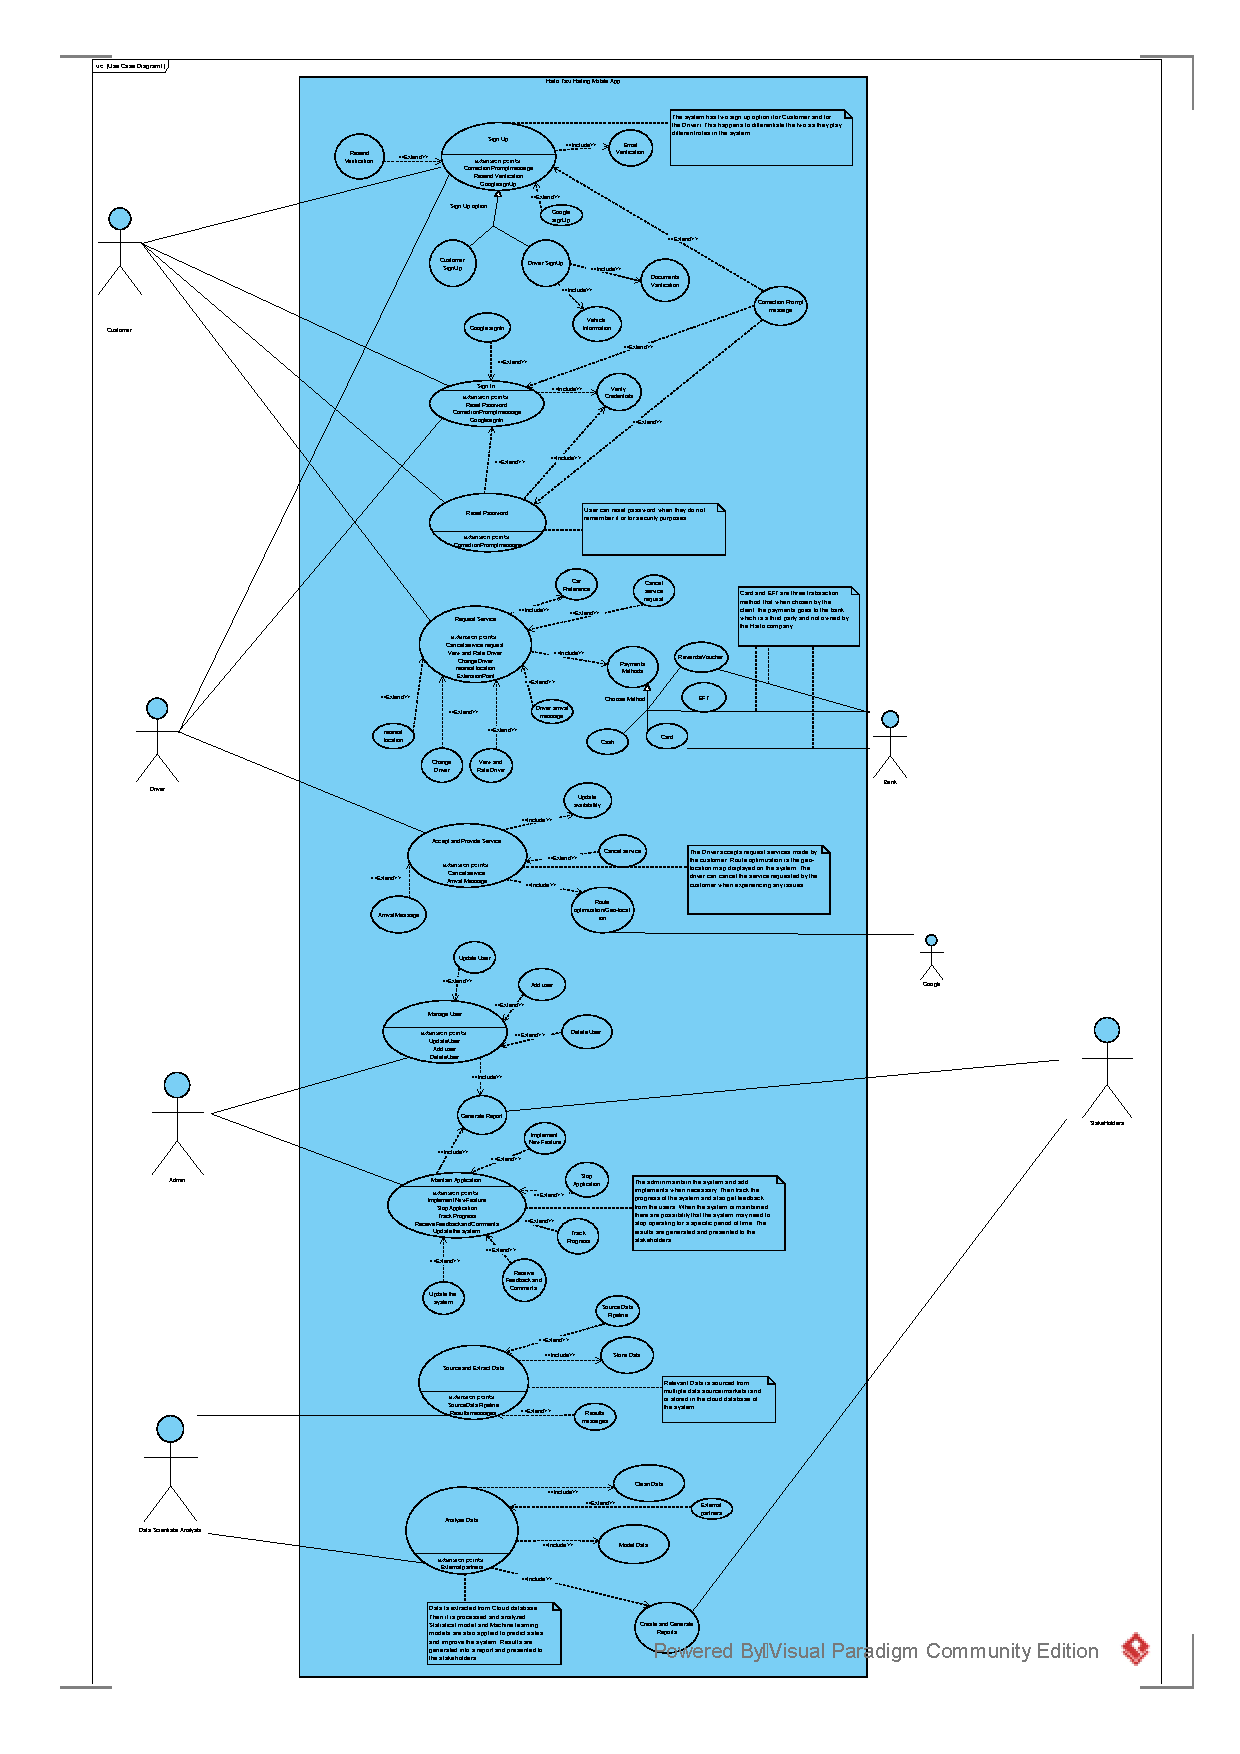
\includepdf [pages=-]{UsecaseNo2.pdf}


\section*{\\\\5. TRACEABILITY MATRIX}

\begin{tabular}{|p{2cm}|p{2cm}|p{1cm}|p{1cm}|p{1cm}|p{1cm}|p{1cm}|p{1cm}|p{1cm}|p{1cm}|p{1cm}|}
     \hline
 \rowcolor{lightgray} \textbf{Functional Requirements} & \textbf{Requirements Rates} & \textbf{U1} & \textbf{U2} & \textbf{U3} & \textbf{U4} & \textbf{U5} & \textbf{U6} & \textbf{U7} & \textbf{U8} & \textbf{U9}\\
 \hline
 \textbf{Totals:} & \textbf{} & \textbf{9} & \textbf{5} & \textbf{4} & \textbf{3} & \textbf{3} & \textbf{3} & \textbf{3} & \textbf{3} & \textbf{3}\\
 \hline
 \textbf{FR1.3} & \textbf{3} & \textbf{X} & \textbf{} & \textbf{X} & \textbf{} & \textbf{} & \textbf{} & \textbf{} & \textbf{} & \textbf{}\\
 \hline
 \textbf{FR1.5} & \textbf{3} & \textbf{X} & \textbf{} & \textbf{} & \textbf{} & \textbf{} & \textbf{} & \textbf{} & \textbf{} & \textbf{}\\
 \hline
 \textbf{FR1.6} & \textbf{5} & \textbf{X} & \textbf{} & \textbf{} & \textbf{} & \textbf{} & \textbf{} & \textbf{} & \textbf{} & \textbf{}\\
 \hline
 \textbf{FR2.7} & \textbf{4} & \textbf{} & \textbf{X} & \textbf{} & \textbf{X} & \textbf{} & \textbf{} & \textbf{} & \textbf{} & \textbf{}\\
 \hline
 \textbf{FR2.9} & \textbf{2} & \textbf{X} & \textbf{X} & \textbf{} & \textbf{} & \textbf{} & \textbf{} & \textbf{} & \textbf{} & \textbf{}\\
 \hline
 \textbf{FR4.1} & \textbf{4} & \textbf{} & \textbf{} & \textbf{} & \textbf{X} & \textbf{X} & \textbf{} & \textbf{} & \textbf{} & \textbf{}\\
 \hline
 \textbf{FR6.3} & \textbf{4} & \textbf{} & \textbf{} & \textbf{} & \textbf{} & \textbf{} & \textbf{X} & \textbf{X} & \textbf{} & \textbf{}\\
 \hline
 \textbf{FR7.3} & \textbf{4} & \textbf{} & \textbf{} & \textbf{} & \textbf{} & \textbf{} & \textbf{} & \textbf{X} & \textbf{X} & \textbf{X}\\
 \hline
 \hline
 \textbf{CR.1} & \textbf{4} & \textbf{X} & \textbf{X} & \textbf{X} & \textbf{X} & \textbf{X} & \textbf{} & \textbf{} & \textbf{} & \textbf{}\\
 \hline
 \textbf{CR.2} & \textbf{4} & \textbf{X} & \textbf{X} & \textbf{X} & \textbf{} & \textbf{} & \textbf{} & \textbf{} & \textbf{} & \textbf{}\\
 \hline
 \textbf{CR.3} & \textbf{4} & \textbf{X} & \textbf{} & \textbf{} & \textbf{} & \textbf{} & \textbf{X} & \textbf{} & \textbf{} & \textbf{}\\
 \hline
 \textbf{CR.6} & \textbf{4} & \textbf{X} & \textbf{} & \textbf{} & \textbf{} & \textbf{} & \textbf{X} & \textbf{X} & \textbf{X} & \textbf{X}\\
 \hline
 \textbf{CR.8} & \textbf{4} & \textbf{X} & \textbf{X} & \textbf{X} & \textbf{} & \textbf{X} & \textbf{} & \textbf{} & \textbf{X} & \textbf{X}\\
 \hline
\end{tabular}

%----------------------------------------UML---------------------------------------
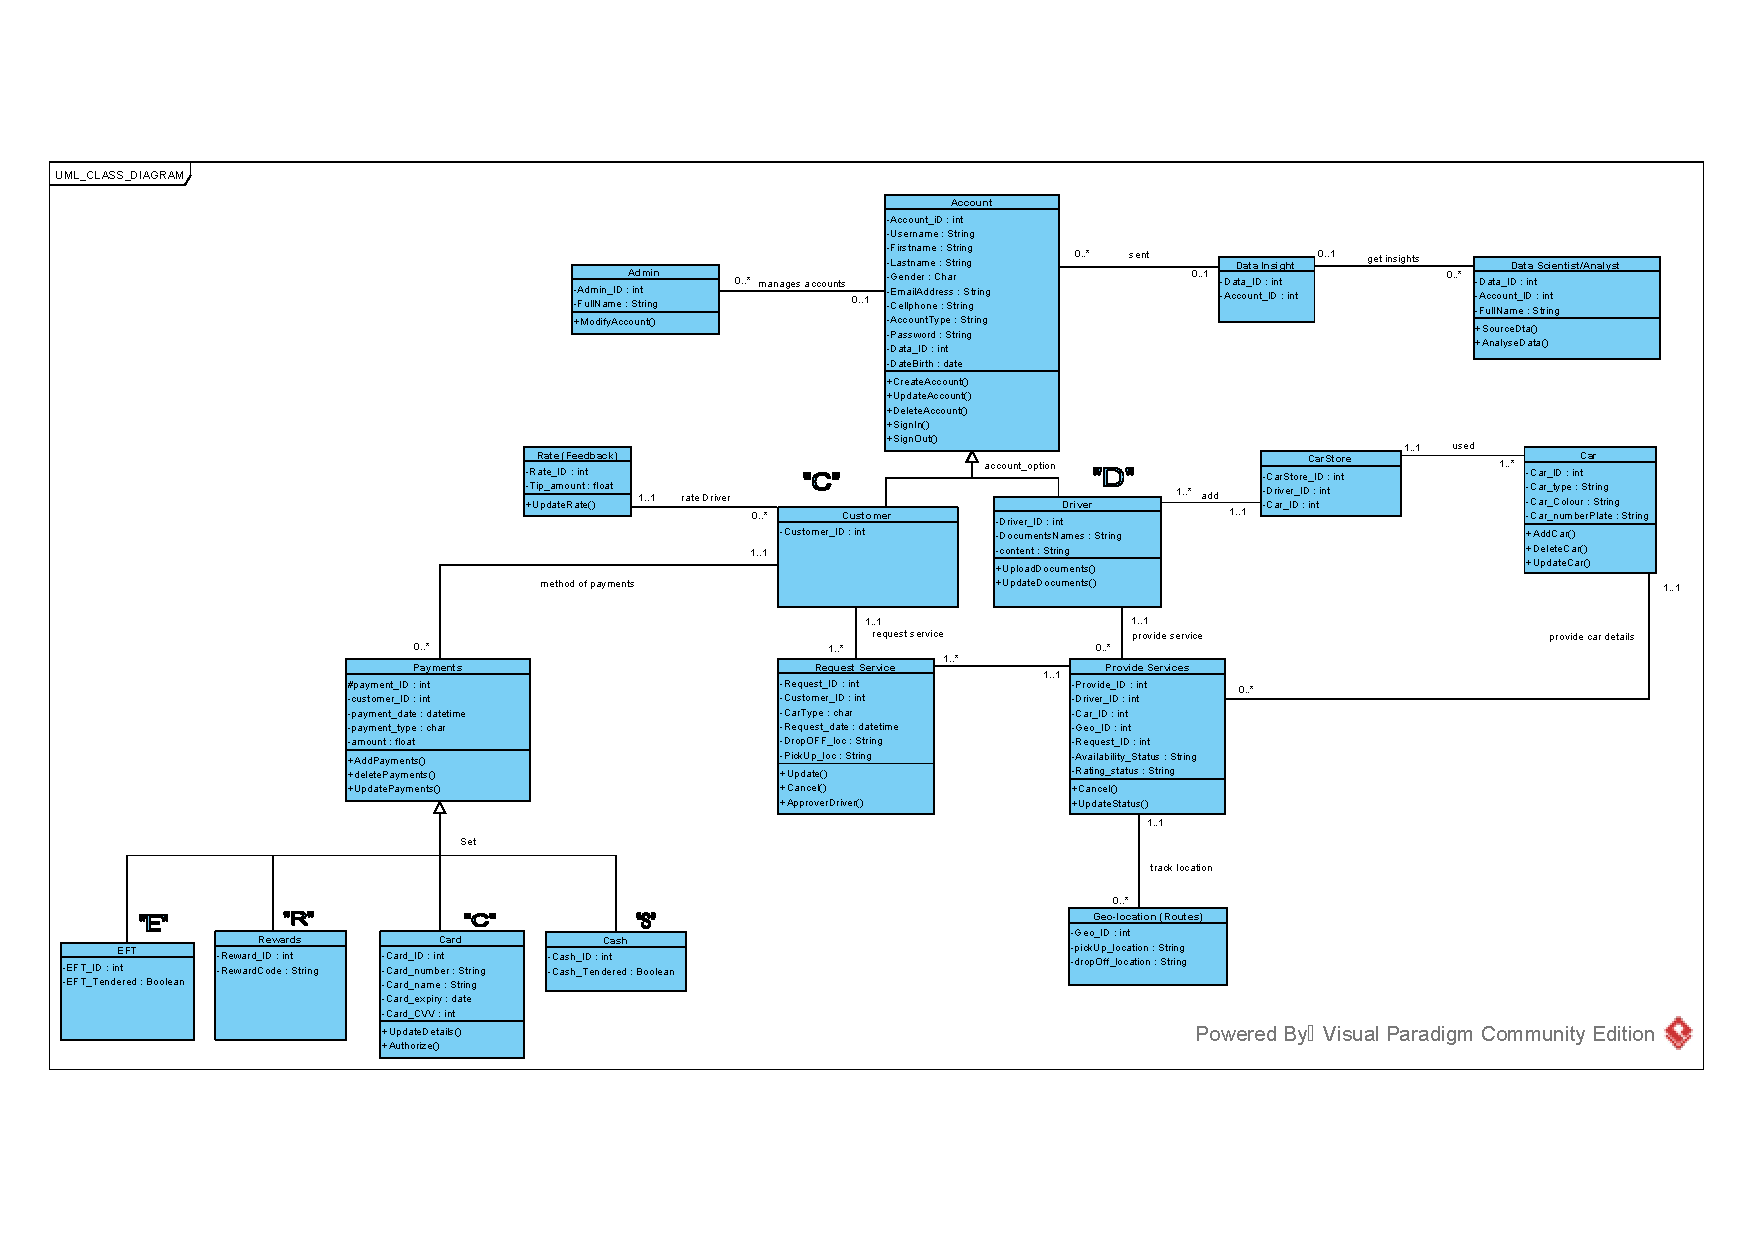
\includepdf [pages=-]{UML diagram_rotated.pdf}
%----------------------------------------Non Functional---------------------------------------


\newpage
\section*{4. HIGH-LEVEL NON-FUNCTIONAL REQUIREMENTS:}

\begin{tabular}{ |p{4cm}|p{12cm}| }
 \hline
 \rowcolor{lightgray} \textbf{PIECES CATEGORIES (REQUIREMENTS)} & \textbf{DESCRIPTION}\\
 \hline
 \textbf{CR1.Performance}   & The application should respond quickly to administrative activities. When connecting with the database through APIs for payments, sign-ups, sign-ins, or password recovery, the application should listen and respond quickly.\\
  \hline
 \textbf{CR2.Security} &   Validations should occur during sign-up, sign-in, and password recovery. Sensitive data should be preserved and encrypted before being saved to a database or other data repository. There should be access controls in place, as well as regular security audits. When unknown situations occur, the system should be capable of responding promptly. \\
  \hline
 \textbf{CR3.Scalability} & The programme should be capable of handling vast quantities of data going through databases, listening to data from the database, updating data, and accommodating an increasing number of users, service requests, and accepting service requests.\\
 \hline
 \textbf{CR4.Reliability} &The system should be reliable and stable, with minimal downtime and no data loss. The system should shut down less frequently, and services should always be available at any time. There should be limited delays when requesting services and no incorrect payments.\\
 \hline
 \textbf{CR5.Compatibility}&   The programme should be compatible with a variety of mobile operating systems, particularly for IOS and Android.\\
 \hline
 \textbf{CR6.Compliance}& To ensure data protection, the system ought to adhere to the legislation of the country (location) where the services are provided, as well as data privacy regulations.\\
 \hline
 \textbf{CR7.User Interface}& The system should be user-friendly and simple to use, with typefaces that may be modified for better reading. The system should be simple to use, available across several devices, and include audio.
\\
 \hline
 \textbf{CR8.Error Handling}& The system should have the capacity to handle unexpected errors and record them so that maintainers can locate where the error occurred while minimising hours of downtime.
\\
 \hline
 \textbf{CR9.Maintainability}& The code should be fully documented and written to allow adaptation to subsequent updates and errors, as well as easy navigation. There should be system documentation that serves as a roadmap for changes and maintenance.
\\
 \hline
 
\end{tabular}


\begin{tabular}{ |p{4cm}|p{12cm}| }
 \hline
 \rowcolor{lightgray} \textbf{PIECES CATEGORIES (REQUIREMENTS)} & \textbf{DESCRIPTION}\\
 \hline
 \textbf{CR10.Accessibility}& The system should be accessible to all users with impairments by allowing them to modify the system's colours to assist their eyesight and, if possible, resize the text.
 \\
 \hline
 \textbf{CR11.Localization}& The system should use English as a general language, as well as other spoken languages in the area where it will operate. The system should accept the money of the location in which it operates.
\\
 \hline
\end{tabular}




%-------------------------------------------------------------------------------
% REFERENCES
%-------------------------------------------------------------------------------
\newpage

\bibliographystyle{plain}
\bibliography{MyReferences}

\end{document}

%-------------------------------------------------------------------------------
% SNIPPETS
%-------------------------------------------------------------------------------

%\begin{figure}[!ht]
%	\centering
%	\includegraphics[width=0.8\textwidth]{file_name}
%	\caption{}
%	\centering
%	\label{label:file_name}
%\end{figure}

%\begin{figure}[!ht]
%	\centering
%	\includegraphics[width=0.8\textwidth]{graph}
%	\caption{Blood pressure ranges and associated level of hypertension (American Heart Association, 2013).}
%	\centering
%	\label{label:graph}
%\end{figure}

%\begin{wrapfigure}{r}{0.30\textwidth}
%	\vspace{-40pt}
%	\begin{center}
%		\includegraphics[width=0.29\textwidth]{file_name}
%	\end{center}
%	\vspace{-20pt}
%	\caption{}
%	\label{label:file_name}
%\end{wrapfigure}

%\begin{wrapfigure}{r}{0.45\textwidth}
%	\begin{center}
%		\includegraphics[width=0.29\textwidth]{manometer}
%	\end{center}
%	\caption{Aneroid sphygmomanometer with stethoscope (Medicalexpo, 2012).}
%	\label{label:manometer}
%\end{wrapfigure}

%\begin{table}[!ht]\footnotesize
%	\centering
%	\begin{tabular}{cccccc}
%	\toprule
%	\multicolumn{2}{c} {Pearson's correlation test} & \multicolumn{4}{c} {Independent t-test} \\
%	\midrule	
%	\multicolumn{2}{c} {Gender} & \multicolumn{2}{c} {Activity level} & \multicolumn{2}{c} {Gender} \\
%	\midrule
%	Males & Females & 1st level & 6th level & Males & Females \\
%	\midrule
%	\multicolumn{2}{c} {BMI vs. SP} & \multicolumn{2}{c} {Systolic pressure} & \multicolumn{2}{c} {Systolic Pressure} \\
%	\multicolumn{2}{c} {BMI vs. DP} & \multicolumn{2}{c} {Diastolic pressure} & \multicolumn{2}{c} {Diastolic pressure} \\
%	\multicolumn{2}{c} {BMI vs. MAP} & \multicolumn{2}{c} {MAP} & \multicolumn{2}{c} {MAP} \\
%	\multicolumn{2}{c} {W:H ratio vs. SP} & \multicolumn{2}{c} {BMI} & \multicolumn{2}{c} {BMI} \\
%	\multicolumn{2}{c} {W:H ratio vs. DP} & \multicolumn{2}{c} {W:H ratio} & \multicolumn{2}{c} {W:H ratio} \\
%	\multicolumn{2}{c} {W:H ratio vs. MAP} & \multicolumn{2}{c} {\% Body fat} & \multicolumn{2}{c} {\% Body fat} \\
%	\multicolumn{2}{c} {} & \multicolumn{2}{c} {Height} & \multicolumn{2}{c} {Height} \\
%	\multicolumn{2}{c} {} & \multicolumn{2}{c} {Weight} & \multicolumn{2}{c} {Weight} \\
%	\multicolumn{2}{c} {} & \multicolumn{2}{c} {Heart rate} & \multicolumn{2}{c} {Heart rate} \\
%	\bottomrule
%	\end{tabular}
%	\caption{Parameters that were analysed and related statistical test performed for current study. BMI - body mass index; SP - systolic pressure; DP - diastolic pressure; MAP - mean arterial pressure; W:H ratio - waist to hip ratio.}
%	\label{label:tests}
%\end{table}